\subsection{Semiconductor Parameter Analyzer}

\subsubsection{\texorpdfstring{$I_{DS}$ vs. $V_{DS}$ Characteristics for various $V_{GS}$}{Dump to Source Current vs Voltage Characteristics for various Gate to Source Voltages}}

First we will look at the MOSFET's three terminal characteristics:

\begin{figure}[ht]
    \centering
    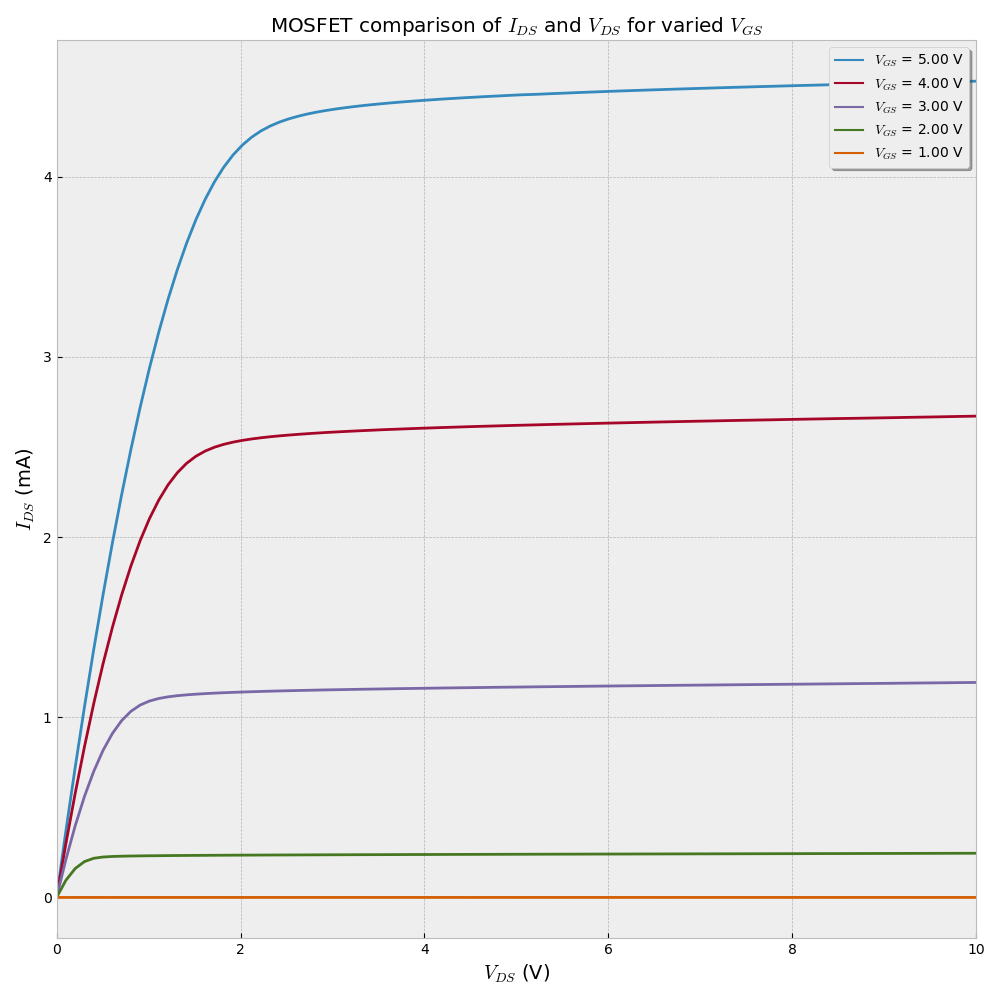
\includegraphics[width=.95\linewidth]{figures/characteristic_nothing.png}
    \caption{The characteristic graphs of $I_{DS}$ vs. $V_{DS}$ for several differing values of $V_{GS}$. }
    \label{fig:characteristic}
\end{figure}

\clearpage

We also view these three terminal characteristics through the Agilent Software, which is shown here:

\begin{figure}[ht]
    \centering
    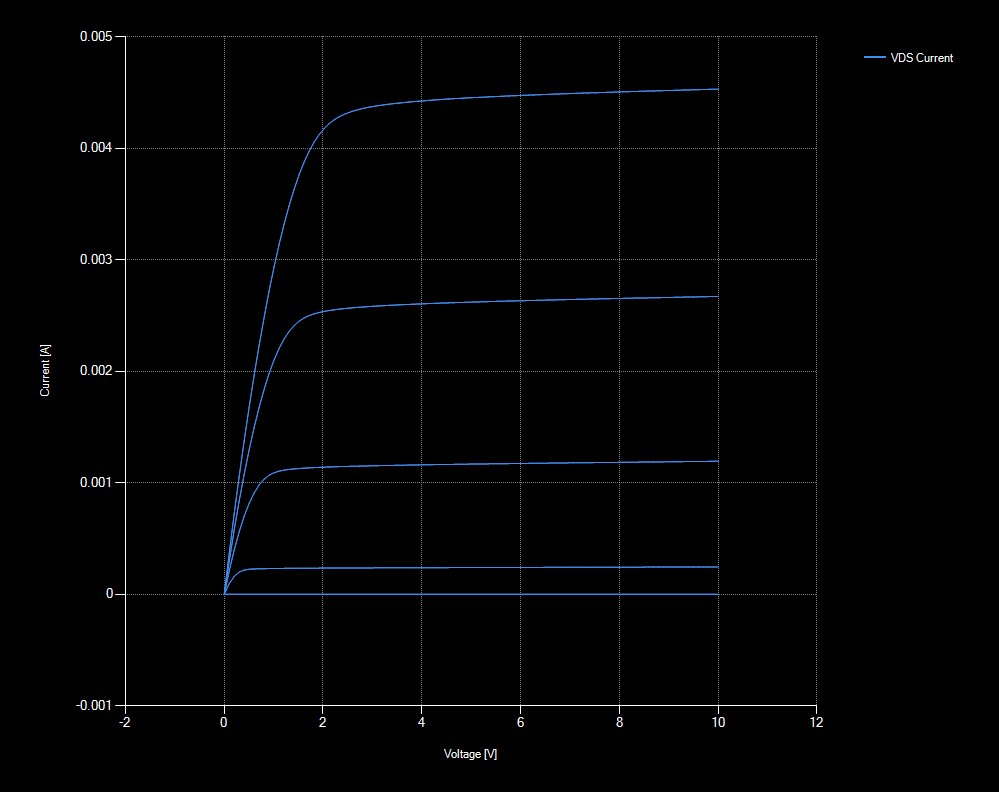
\includegraphics[width=.95\linewidth]{figures/ECE331_Lab3_Data421V1}
    \caption{The characteristic graphs of $I_{DS}$ vs. $V_{DS}$ for several differing values of $V_{GS}$. Shown with in-lab software }
    \label{fig:characteristic_inlab}
\end{figure}

From these graphs we can calculate two important characteristics, these are the MOSFET output resistance $r_o$ and the trans conductance $g_m$.

We note that we can calculate the output resistance by taking two points along a single $V_{GS}$ (The points taken are shown in Figure \ref{fig:VGS_varied}) through $r_o = ( \frac{\partial I_{DS}}{\partial V_{DS}}|_{V_{GS} = constant}$)$^{-1}$. We simply use the delta between the markers where $\Delta V_{DS} \,= \,3.23\; V$  and $\Delta I_{DS} \,= \,75.77\;\mu A$ where $V_{GS}\, = \, 5.00 V$. Therefore $r_o \, = \, 42.63 \;k\Omega$.

We then calculate transconductance $g_m$, where this is defined as $g_m = \frac{\partial I_{DS}}{\partial V_{GS}}|_{V_{DS} = constant}$. The points taken are shown in Figure \ref{fig:VGS_constant}, where the deltas $\Delta V_{GS} \,= \,1.00\; V$  and $\Delta I_{DS} \,= \,1.815\;m A$ where $V_{DS}\, = \, 3.73 V$. Therefore $g_m \, = \, 1.815 \;mS$.

\clearpage

To find the early voltage, the saturation portion of the curves are fitted with a linear function and then the x intercept should be the value of the early voltage. The fitting is completed here, with the fit shown in  Figure \ref{fig:characteristic_tight_fit}. Then the intercepts are found in Figure \ref{fig:characteristic_wide_fit}. We see that there is large variation in the values of early voltage, leading to an experimentally found value of $V_E \, = \, -250 \pm 50 V$.

\begin{figure}[ht]
    \centering
    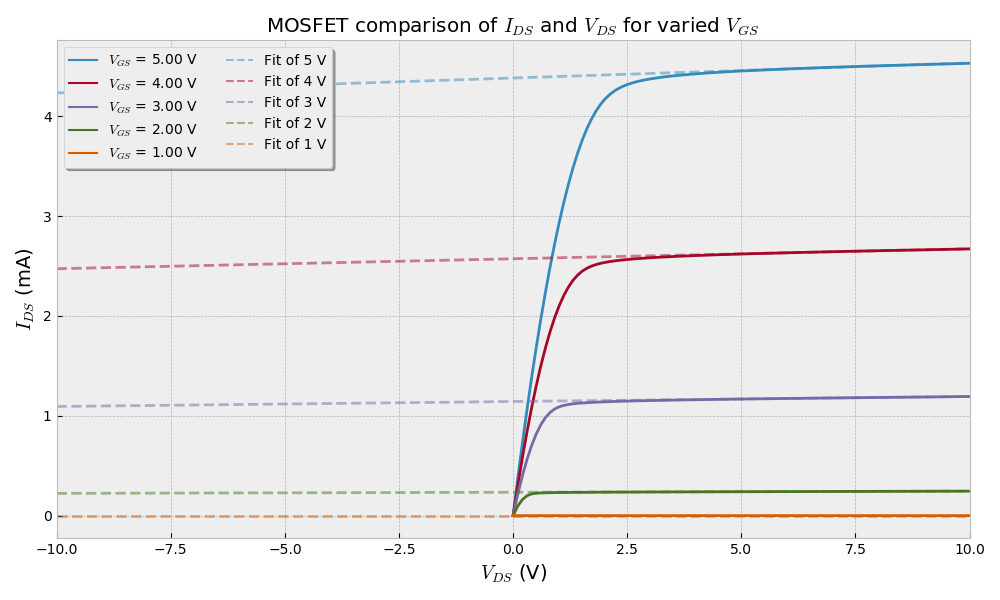
\includegraphics[width=.825\linewidth]{figures/characteristic_tight_fit.png}
    \caption{The characteristic graph with linear fit of saturation portion of curve to show quality of fit.}
    \label{fig:characteristic_tight_fit}
\end{figure}

\begin{figure}[ht]
    \centering
    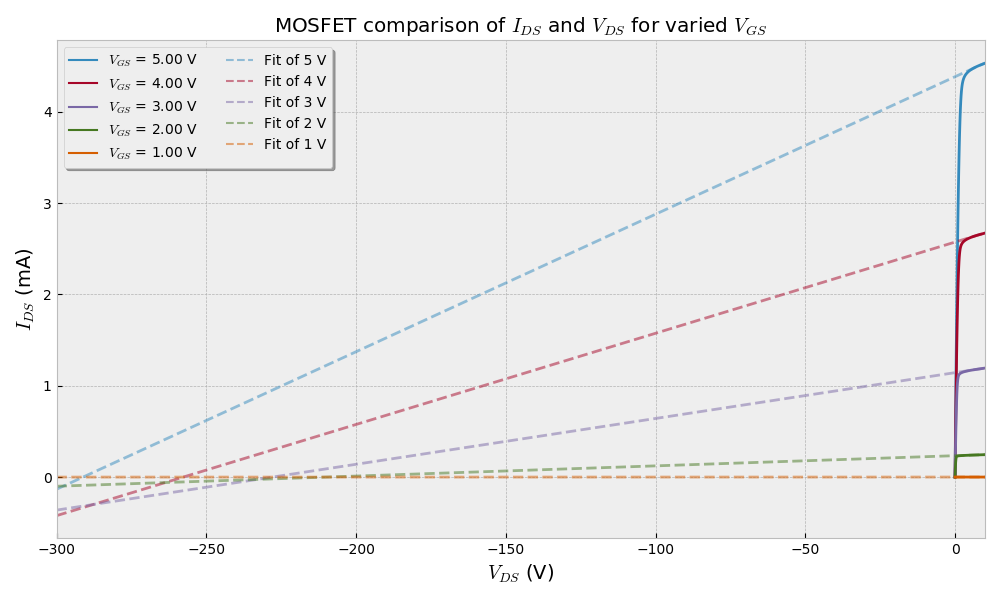
\includegraphics[width=.825\linewidth]{figures/characteristic_wide_fit.png}
    \caption{The characteristic graph with linear fit to show the Early Voltage}
    \label{fig:characteristic_wide_fit}
\end{figure}

\clearpage

To estimate the threshold voltage we graph the value of $I_{DS}$ vs. $V_{GS}$. this is shown in Figure \ref{fig:characteristic_threshold}. Due to the low number of $V_{GS}$ points which are taken, the determination of $V_T$ is a rough approximation. We approximate that it is 1V. This agrees with the found estimated value found during data collection.

\begin{figure}[ht]
    \centering
    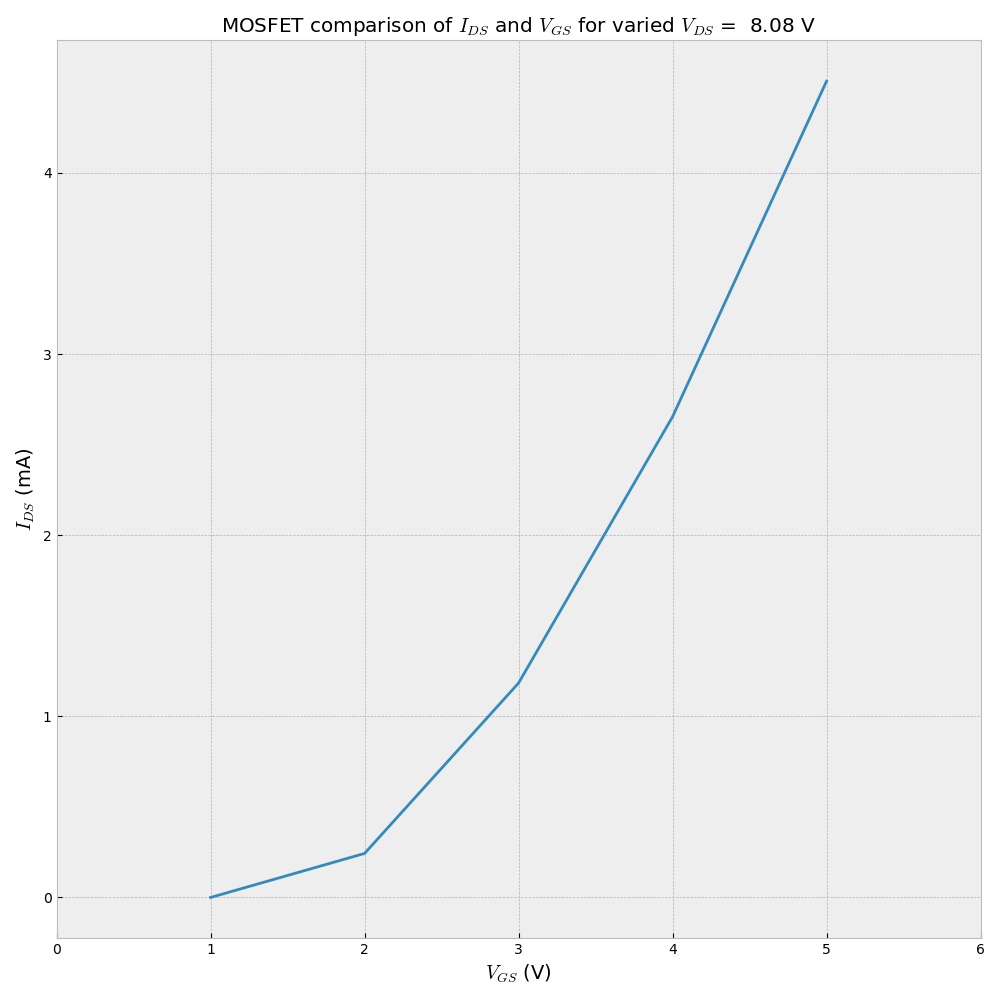
\includegraphics[width=.95\linewidth]{figures/characteristic_threshold.png}
    \caption{The characteristic graph of $I_{DS}$ vs. $V_{GS}$ used for determining the threshold voltage}
    \label{fig:characteristic_threshold}
\end{figure}

\clearpage

Finally for this characteristic graph we show the condition $V_{DS}$ = $V_{GS} - V_T$ which designates the two regions of the graph. These regions correspond to the triode region and the saturation region.

\begin{figure}[ht]
    \centering
    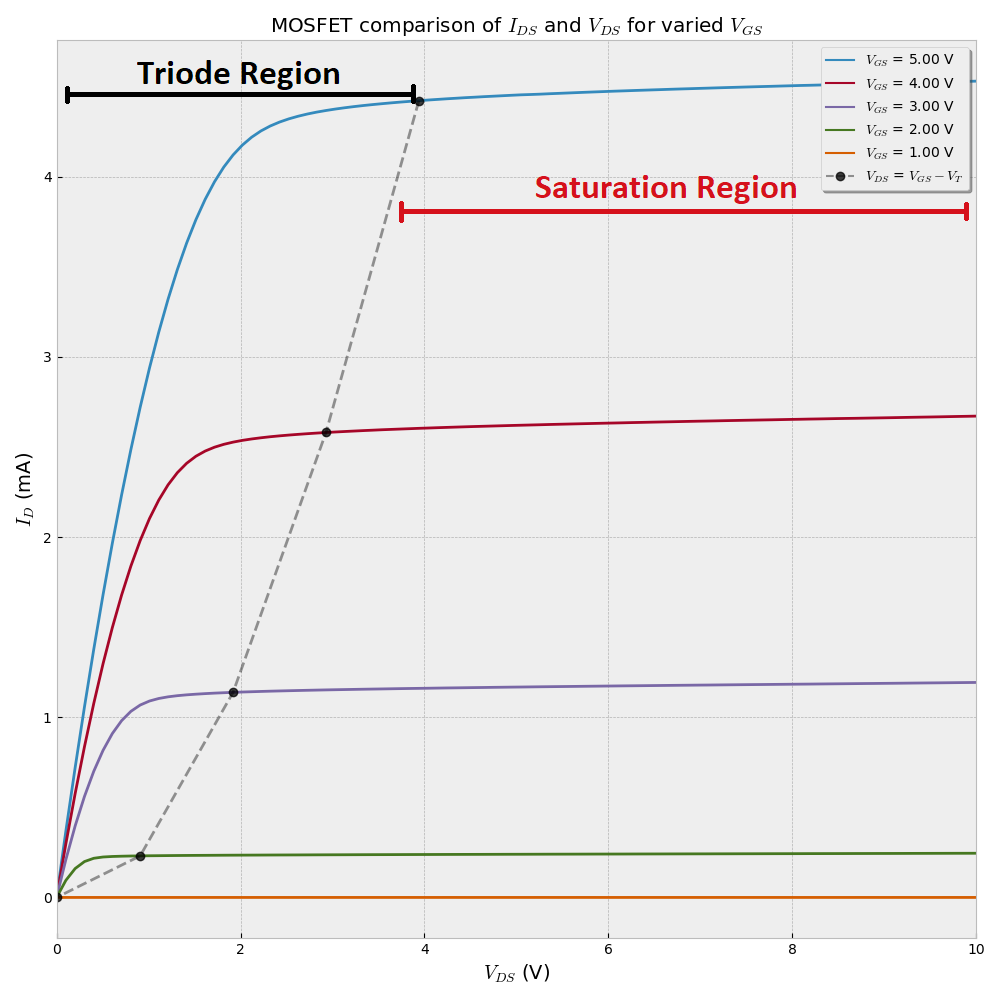
\includegraphics[width=.95\linewidth]{figures/characteristic_intercept_labelled.png}
    \caption{The characteristic graph of $I_{DS}$ vs. $V_{DS}$ with the condition $V_{DS}$ = $V_{GS} - V_T$ inputted and shown on graph}
    \label{fig:characteristic_intercept}
\end{figure}

\clearpage

\subsubsection{\texorpdfstring{$I_{DS}$ vs. $V_{DS}$ Characteristics for various $V_{GS}$ for small $V_{DS}$}{Dump to Source Current vs Small Voltage Characteristics for various Gate to Source Voltages}}

Here we take a look at the characteristic graph of $I_{DS}$ vs. $V_{DS}$ but for small positive and negative values of $V_{DS}$. This is shown in Figure \ref{fig:characteristic_small}. 

We also wish to determine if the MOSFET is behaving as a voltage controlled resistor. We note that a voltage controlled resistor will essentially behave as a passive resistor, except that a third terminal will be able to change the resistance of the device. We note that resistors are linear and in Figure \ref{fig:characteristic_small} we see that the slope of the curve and hence the resistance is controlled by the Gate Voltage. However we also note that the lines are not perfectly linear. These non-linear regions are evidence of distortion in the resistor. We conclude that the MOSFET can be used as a voltage controlled resistor, but care must be taken to avoid distortion effects.

\begin{figure}[ht]
    \centering
    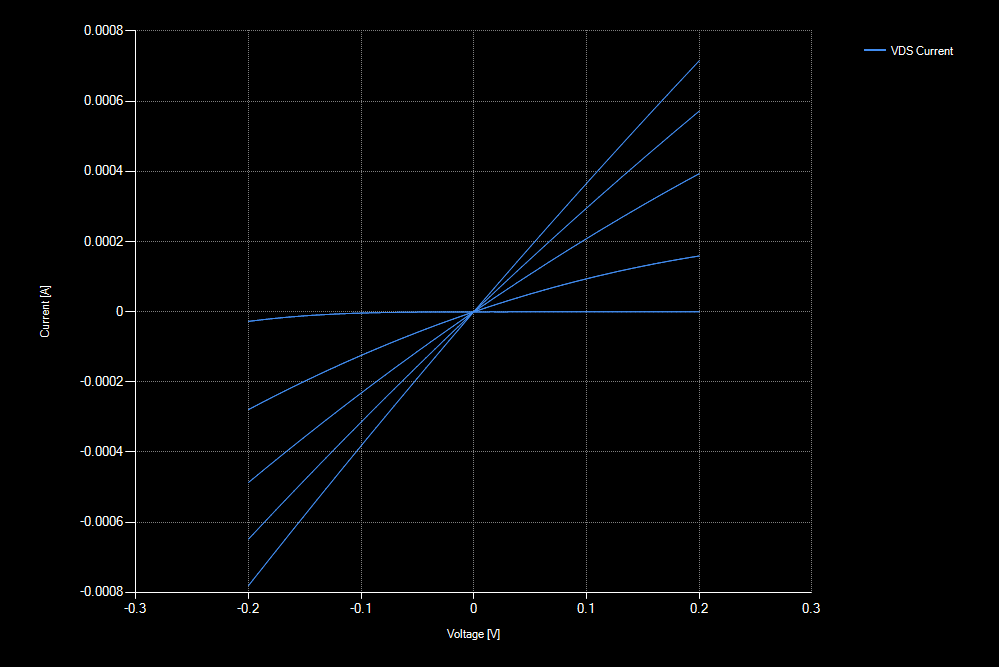
\includegraphics[width=.95\linewidth]{figures/ECE331_Lab3_Data422V1.png}
    \caption{The characteristic graph of $I_{DS}$ vs. $V_{DS}$ with small $V_{DS}$}
    \label{fig:characteristic_small}
\end{figure}